\documentclass[a4paper]{article}

\usepackage{amsmath}
\usepackage{amssymb}
\usepackage{amsthm}
\usepackage{graphicx}
\usepackage{booktabs}
\usepackage[ruled, vlined]{algorithm2e}

\usepackage[backend=biber,style=numeric]{biblatex}
\addbibresource{../references.bib}

\newtheorem{lemma}{Lemma}
\newtheorem{theorem}{Theorem}

\newcommand{\var}{\mathrm{Var}}
\newcommand{\ban}{\mathrm{Ban}}
\newcommand{\diag}{\mathrm{diag}}
\newcommand{\calm}{{\mathcal{M}}}
\newcommand{\calx}{{\mathcal{X}}}
\newcommand{\caln}{{\mathcal{N}}}
\newcommand{\R}{\mathbb{R}}

\begin{document}
\section{DP MCMC Experiments Summary}

\subsection{MMD}
The main metric I used to evaluate MCMC algorithms is maximum mean
discrepancy (MMD). MMD is a statistic that measures the difference
between two distributions, and can be estimated from samples of both
distributions~\cite{GrettonBRSS12}. Using MMD requires choosing a kernel
for the estimation, and the properties of MMD depend on the chosen kernel.
I used the Gaussian kernel, as it requires the distributions to exactly
match reach 0 MMD. The Gaussian kernel requires choosing a kernel width,
which affects how differences in different moments affect the MMD.
I chose the width with the same method as \textcite{GrettonBRSS12},
taking the median between the differences between the two samples,
with the exception that I took a subsample of both samples, and
computed the median between differences of the subsamples. This is necessary
as the MCMC algorithms produce chains of variable lengths.

\subsection{Posteriors}

Figure~\ref{post_plots_fig} shows contour plots of the 2 dimensional
posteriors used for the evaluations. Table~\ref{model_params_table}
contains the parameters of the different models. The variances of
the models did not fit well in the table, so I'll describe them here.
For all banana experiments and 30-dimensional Gauss,
the first component has variance 20, the second has variance 2.5, and
the rest have variance 1. The correlated Gauss has covariance
\[
  \begin{bmatrix}
	1 & 0.999 \\
    0.999 & 1
  \end{bmatrix}.
\]
Note that these are the know variances of the likelihood, not posterior
variances.


\begin{table}[h]
\centering
\caption{
            Model hyperparameters. $n_0$ determines tempering by \(T=\frac{n_0}{n}\).
            For missing $n_0$, \(T = 1\).
            }
\label{model_params_table}
\begin{tabular}{lrrrrr}
\toprule
                   Name &  d &      n &  $n_0$ &     a &  $\sigma^2_0$ \\
\midrule
     Flat banana, d = 2 &  2 & 100000 &        &    20 &          1000 \\
    Flat banana, d = 10 & 10 & 200000 &        &    20 &          1000 \\
 Tempered banana, d = 2 &  2 & 100000 &   1000 &    20 &          1000 \\
Tempered banana, d = 10 & 10 & 200000 &   1000 &    20 &          1000 \\
 High dimensional Gauss & 30 & 200000 &        &     0 &          1000 \\
          Narrow banana &  2 & 150000 &        &   350 &          1000 \\
       Correlated Gauss &  2 & 200000 &        &     0 &           100 \\
                 Circle &  2 & 100000 &        & 1e-05 &               \\
\bottomrule
\end{tabular}
\end{table}


\begin{figure}
  \centering
  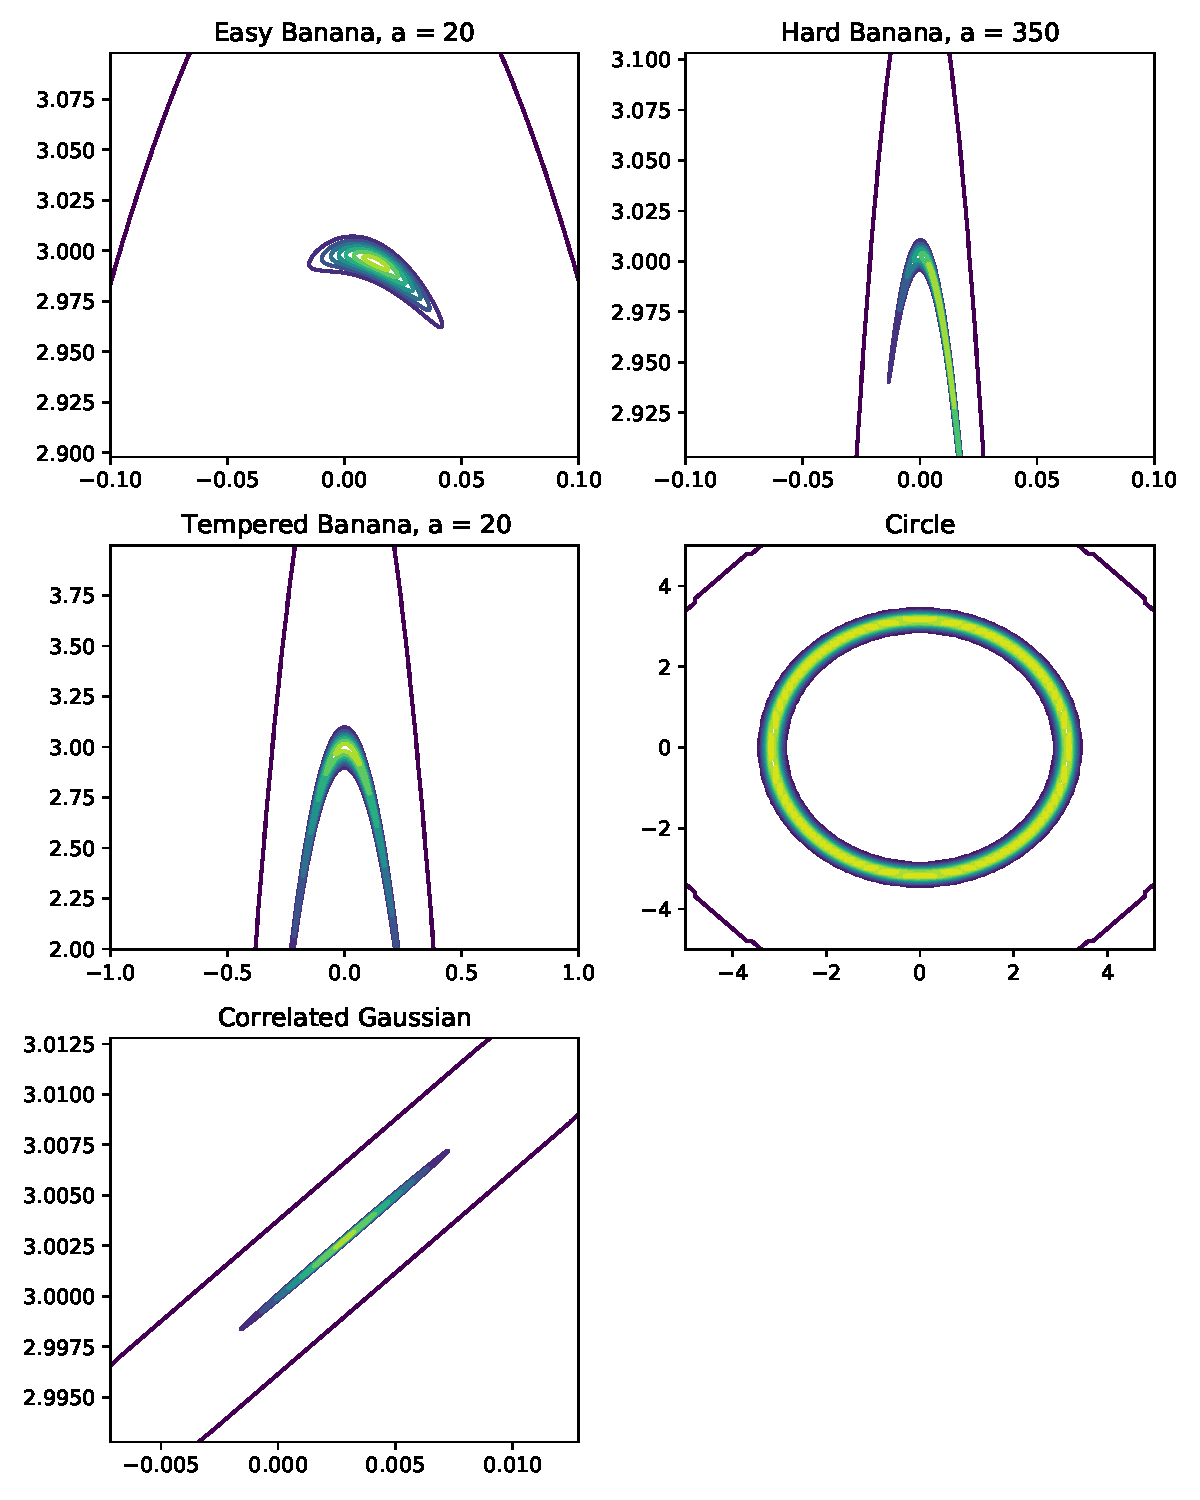
\includegraphics[width=\textwidth]{figures/posterior_plots}
  \caption{Contour plots of the 2-dimensional posteriors}
  \label{post_plots_fig}
\end{figure}

\subsection{Clipping}
Before running experiments on DP MCMC I evaluated the performance of
non-DP random walk Metropolis Hastings and HMC with log likelihood ratio clipping
on the easy banana distribution in both 2 and 10 dimensions. The purpose
of this evaluation is to validate the hypothesis that a small amount
of clipping does not significantly affect the convergence of an
MCMC algorithm, and to find out what that small amount is.

Based on Figure~\ref{clip_fig}, particularly
the bottom row, clipping less than 10\% of the log likelihood ratios
does not significantly affect convergence. Because of this, I tried to
set the clip bounds for the DP experiments to be large enough that
clipping is well under 10\%, when that was possible.

\begin{figure}[h]
  \centering
  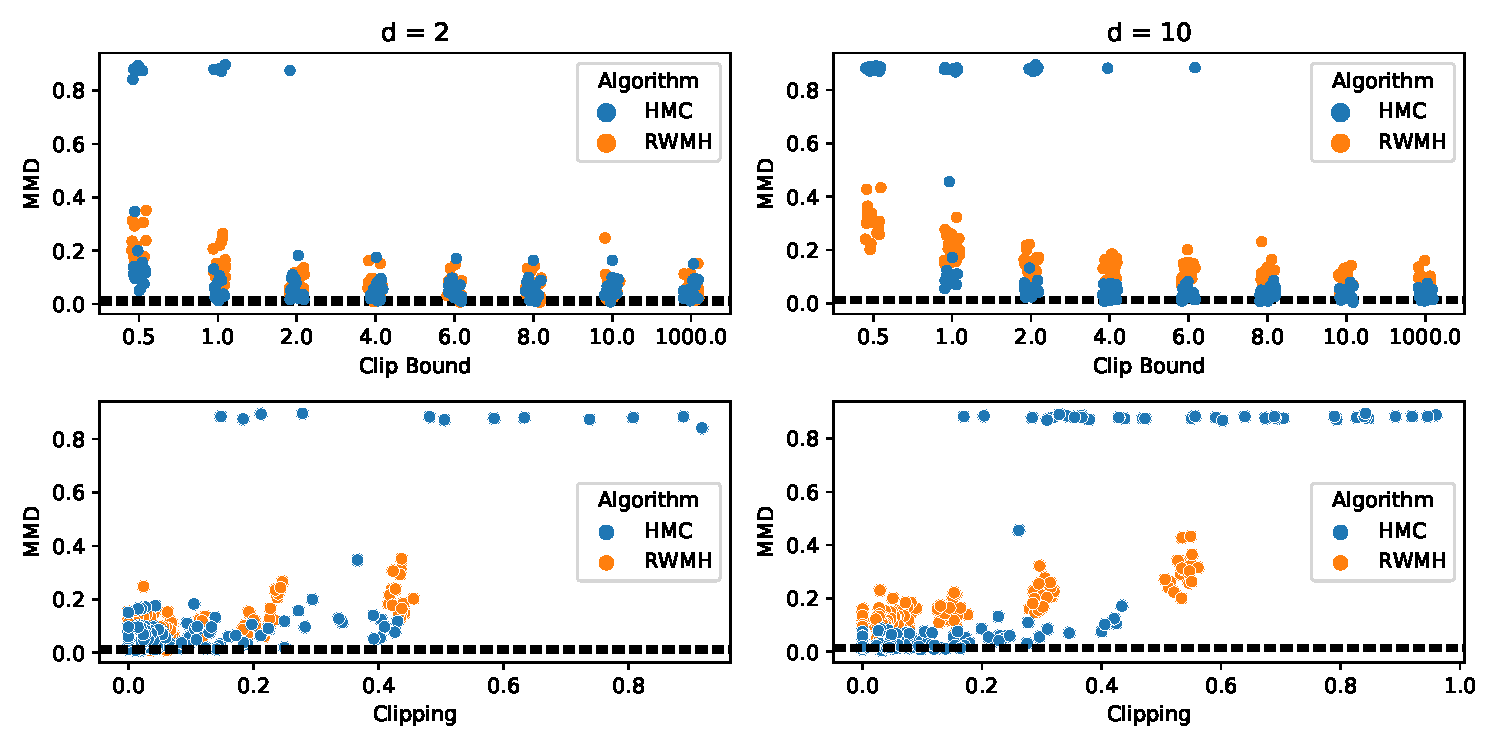
\includegraphics[width=\textwidth]{figures/clipping}
  \caption{Clipping experiment}
  \label{clip_fig}
\end{figure}

\subsection{The algorithms}

The experiments evaluate 6 MCMC algorithms. DP penalty is the
algorithm of \textcite{YildirimE19}, and DP penalty advanced is
DP penalty that only updates one component per sample and
keeps moving in the same direction for each component until a proposal
is rejected, which according to \textcite{YildirimE19} can improve
the performance of the algorithm. Minibatch DP penalty and minibatch DP
penalty advanced are variants of DP penalty (advanced) that only
consider a subsample of the log likelihood ratios for the accept test.
Barker is the algorithm of \textcite{HeikkilaJDH19}.

\subsection{Banana experiments}

All of the DP experiments ran the algorithms 20 times with varying
values of \(\epsilon\). The chains started at a randomly chosen point
centered around the true model parameter values, expect for circle where
the random starting point is centered around \((0, 1)\). The 20 starting
points are the same across algorithms and values of \(\epsilon\).
Table~\ref{model_params_table} column Starting Deviation shows the
the standard deviation of the random starting points.

Figures~\ref{banana_mmd_fig}, \ref{banana_clipping_fig} and
\ref{banana_acceptance_fig} show MMD, clipping and acceptance rate
for the easy and tempered 2 and 10-dimensional banana posteriors.
In the non-tempered experiments, DP HMC is slightly behind DP penalty, but
in the tempered experiment DP HMC is slightly ahead. Clipping is small for
all algorithms except Barker, as the clip bound for Barker is not
adjustable.

\begin{figure}[h]
  \centering
  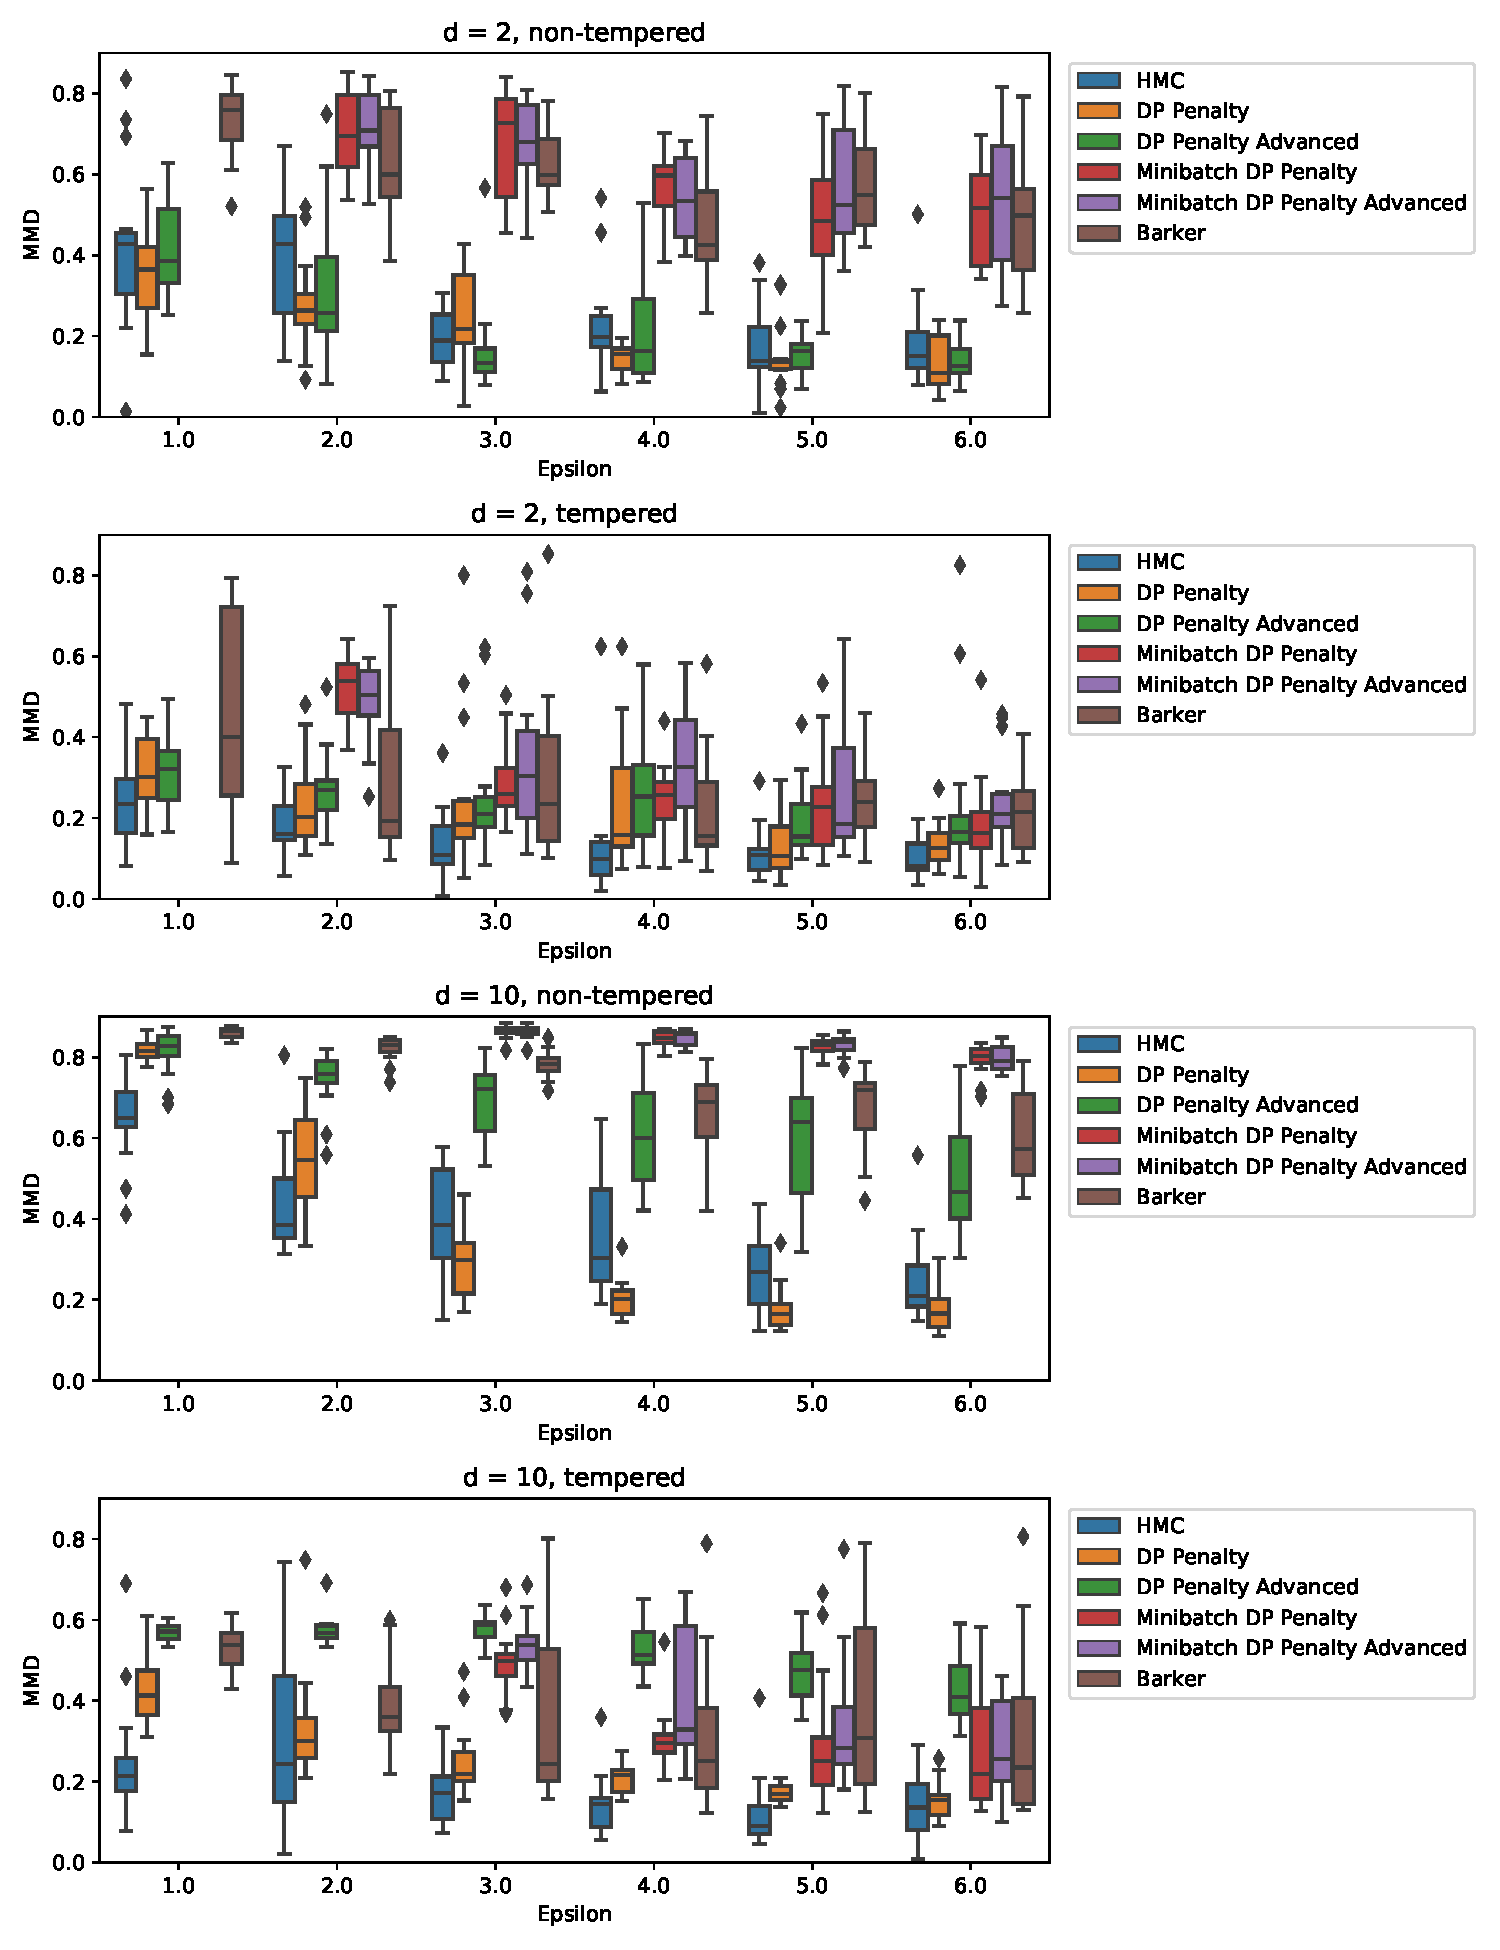
\includegraphics[width=\textwidth]{figures/banana_mmd}
  \caption{Banana experiment MMD}
  \label{banana_mmd_fig}
\end{figure}
\begin{figure}[h]
  \centering
  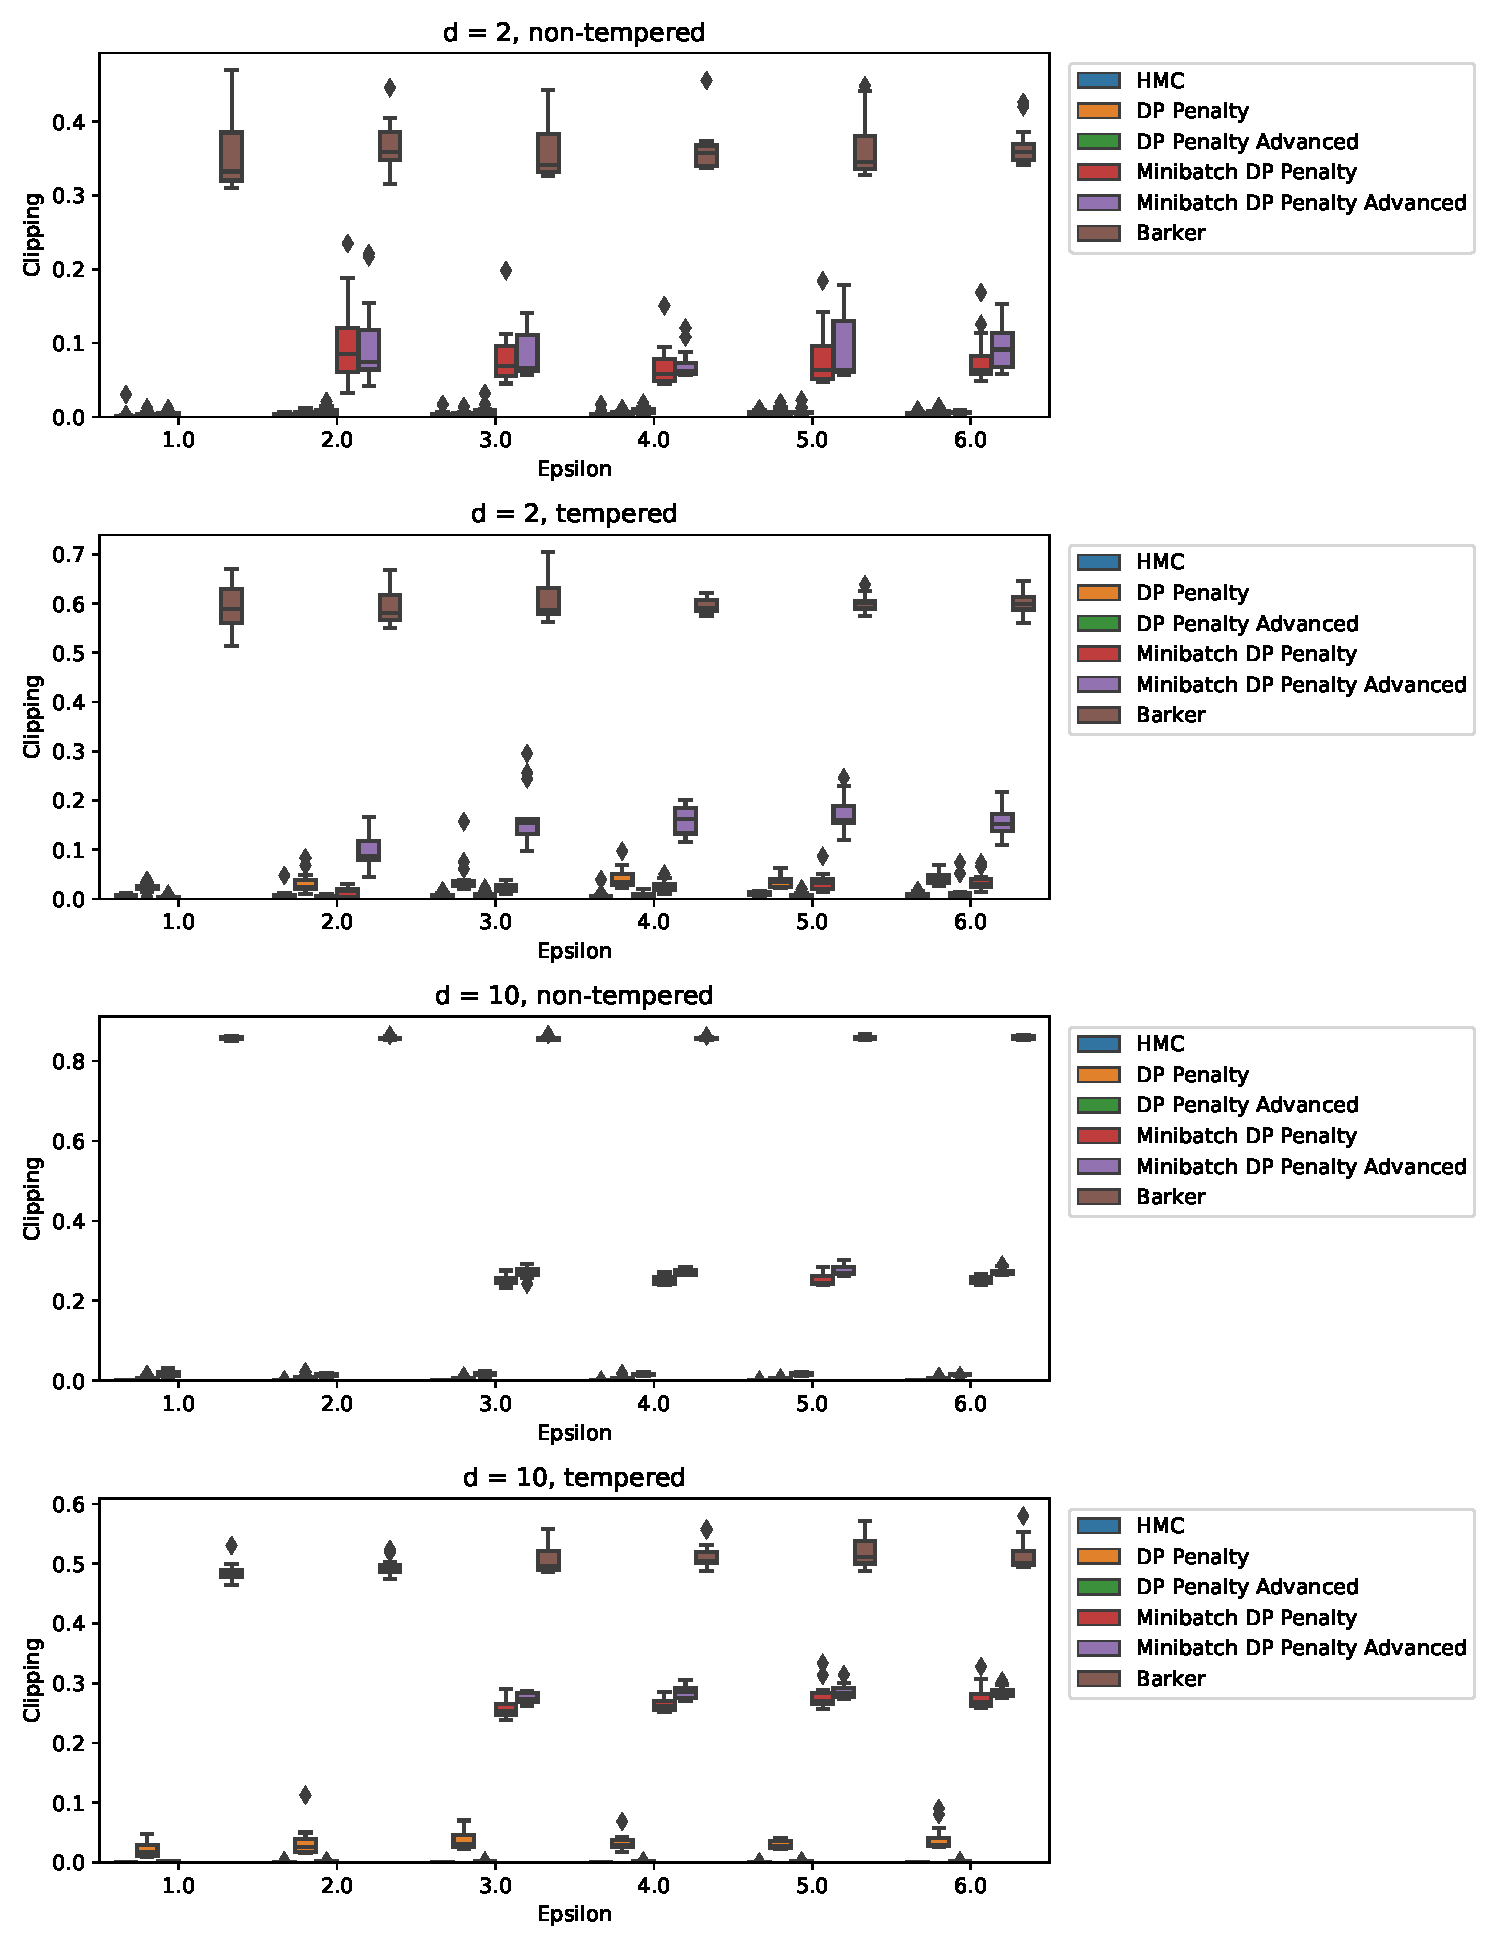
\includegraphics[width=\textwidth]{figures/banana_clipping}
  \caption{Banana experiment clipping}
  \label{banana_clipping_fig}
\end{figure}
\begin{figure}[h]
  \centering
  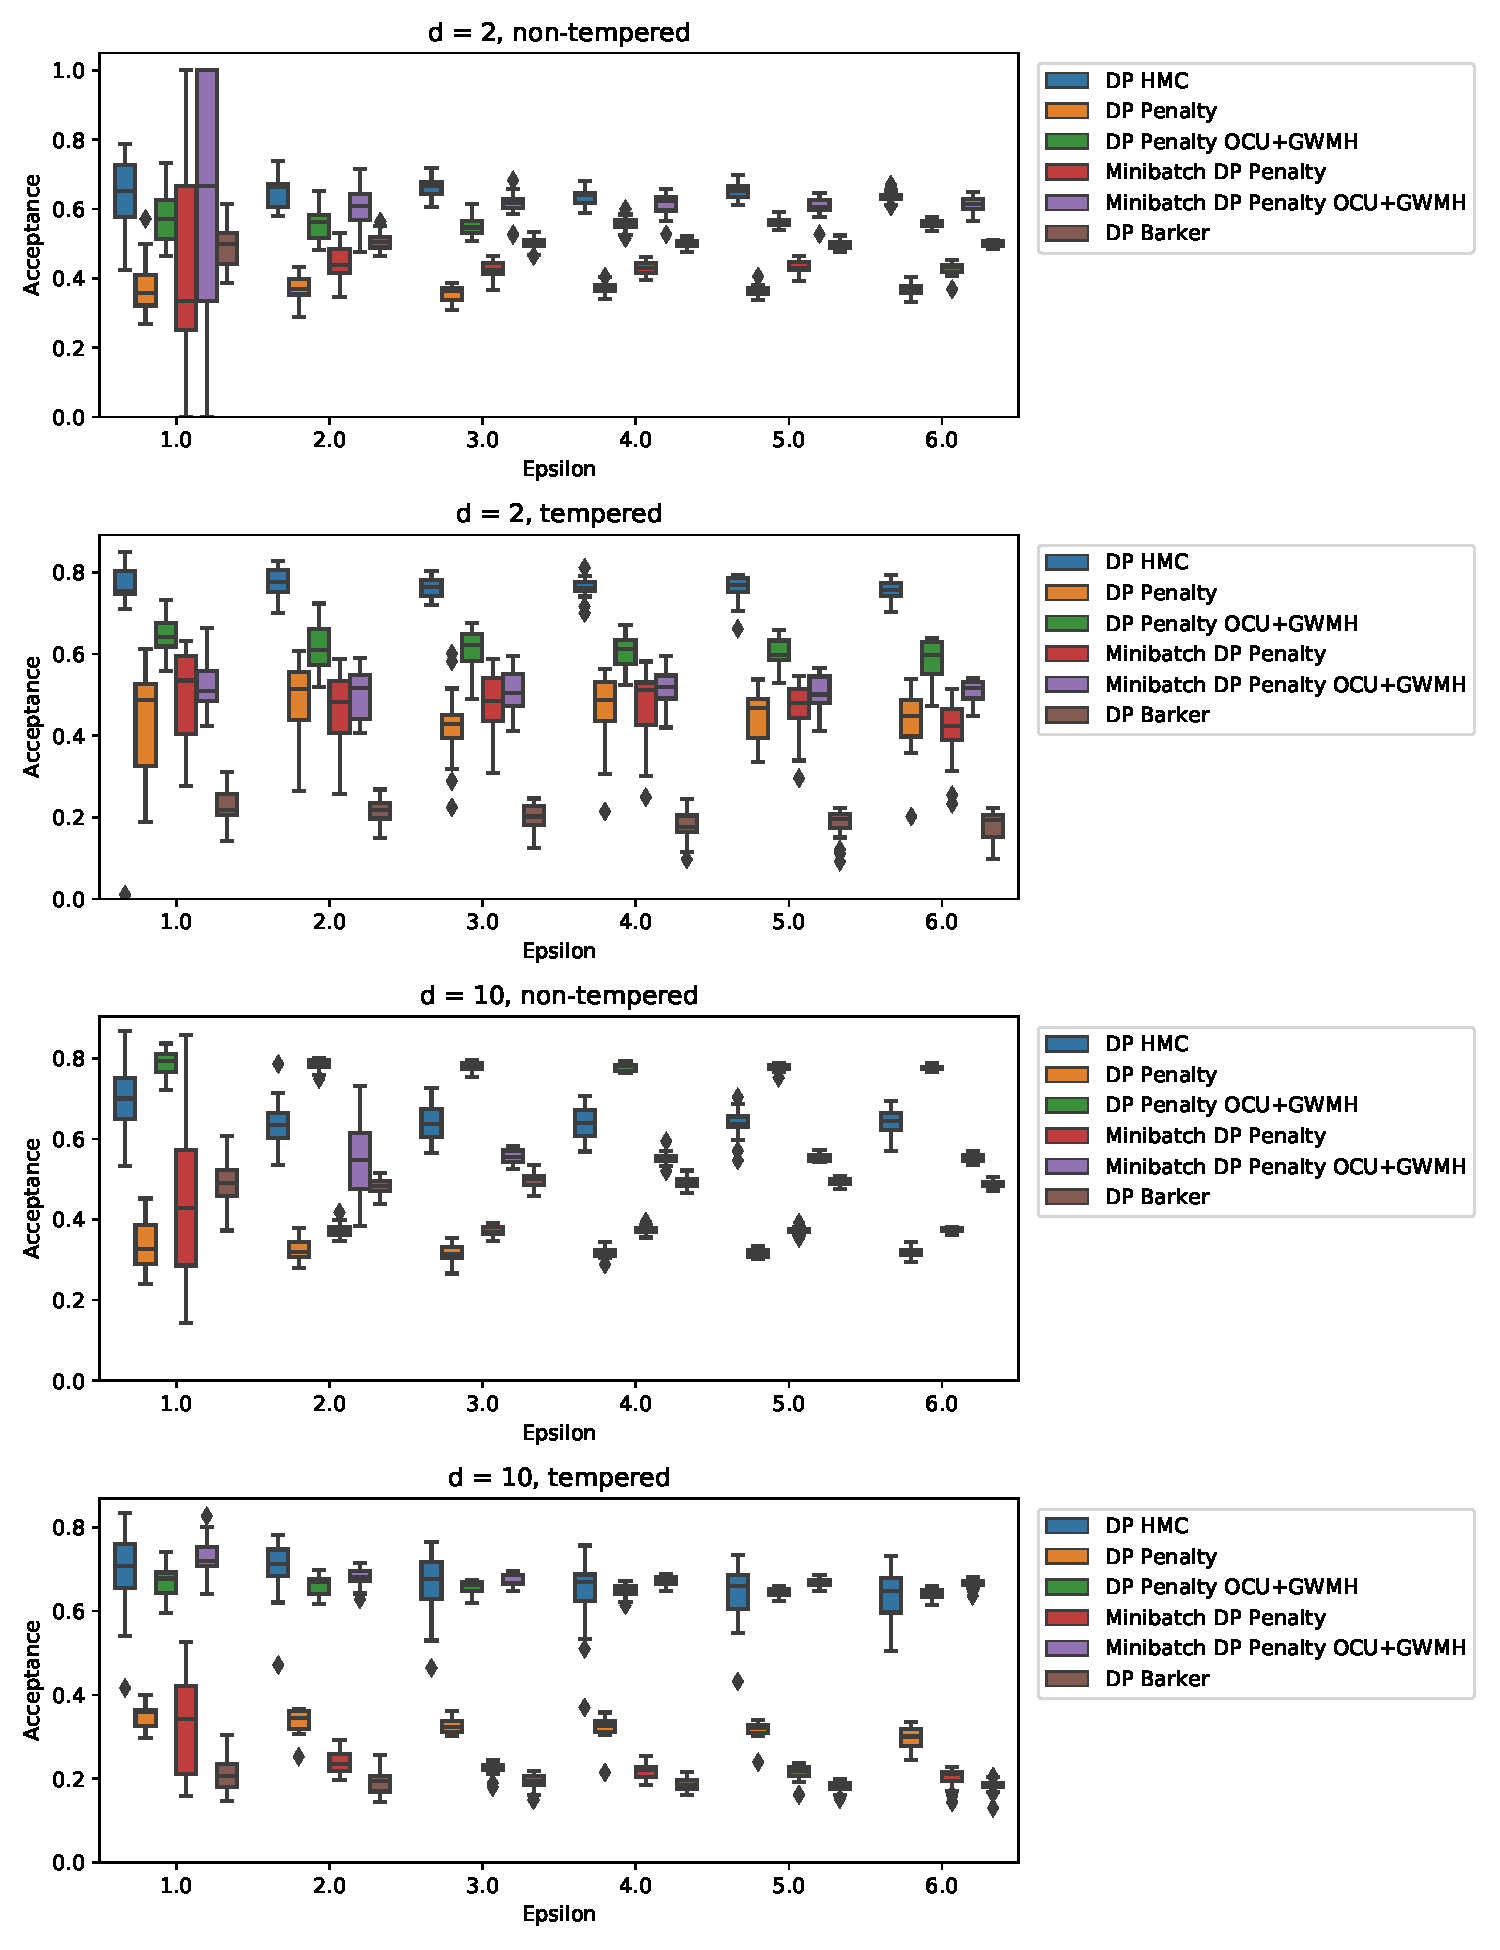
\includegraphics[width=\textwidth]{figures/banana_acceptance}
  \caption{Banana experiment acceptance rate}
  \label{banana_acceptance_fig}
\end{figure}

Figures~\ref{banana_extra_mmd_fig}, \ref{banana_extra_clipping_fig} and
\ref{banana_extra_acceptance_fig} show MMD, clipping and acceptance for
the harder experiments, the 30-dimensional Gaussian, the very curved
hard banana, and the very correlated Gaussian. In the 30-dimensional
Gaussian, HMC is very slightly better than DP penalty, but loses to
DP penalty advanced. With the hard banana, all algorithms perform equally well,
until \(\epsilon = 4\) where DP penalty advanced gets very high variance
for MMD, and larger values of \(\epsilon\) where DP penalty advanced fails
completely. This is likely due to the large amount of clipping for DP penalty
advanced. In the correlated Gaussian, HMC outperforms the other two
algorithms.

\begin{figure}[h]
  \centering
  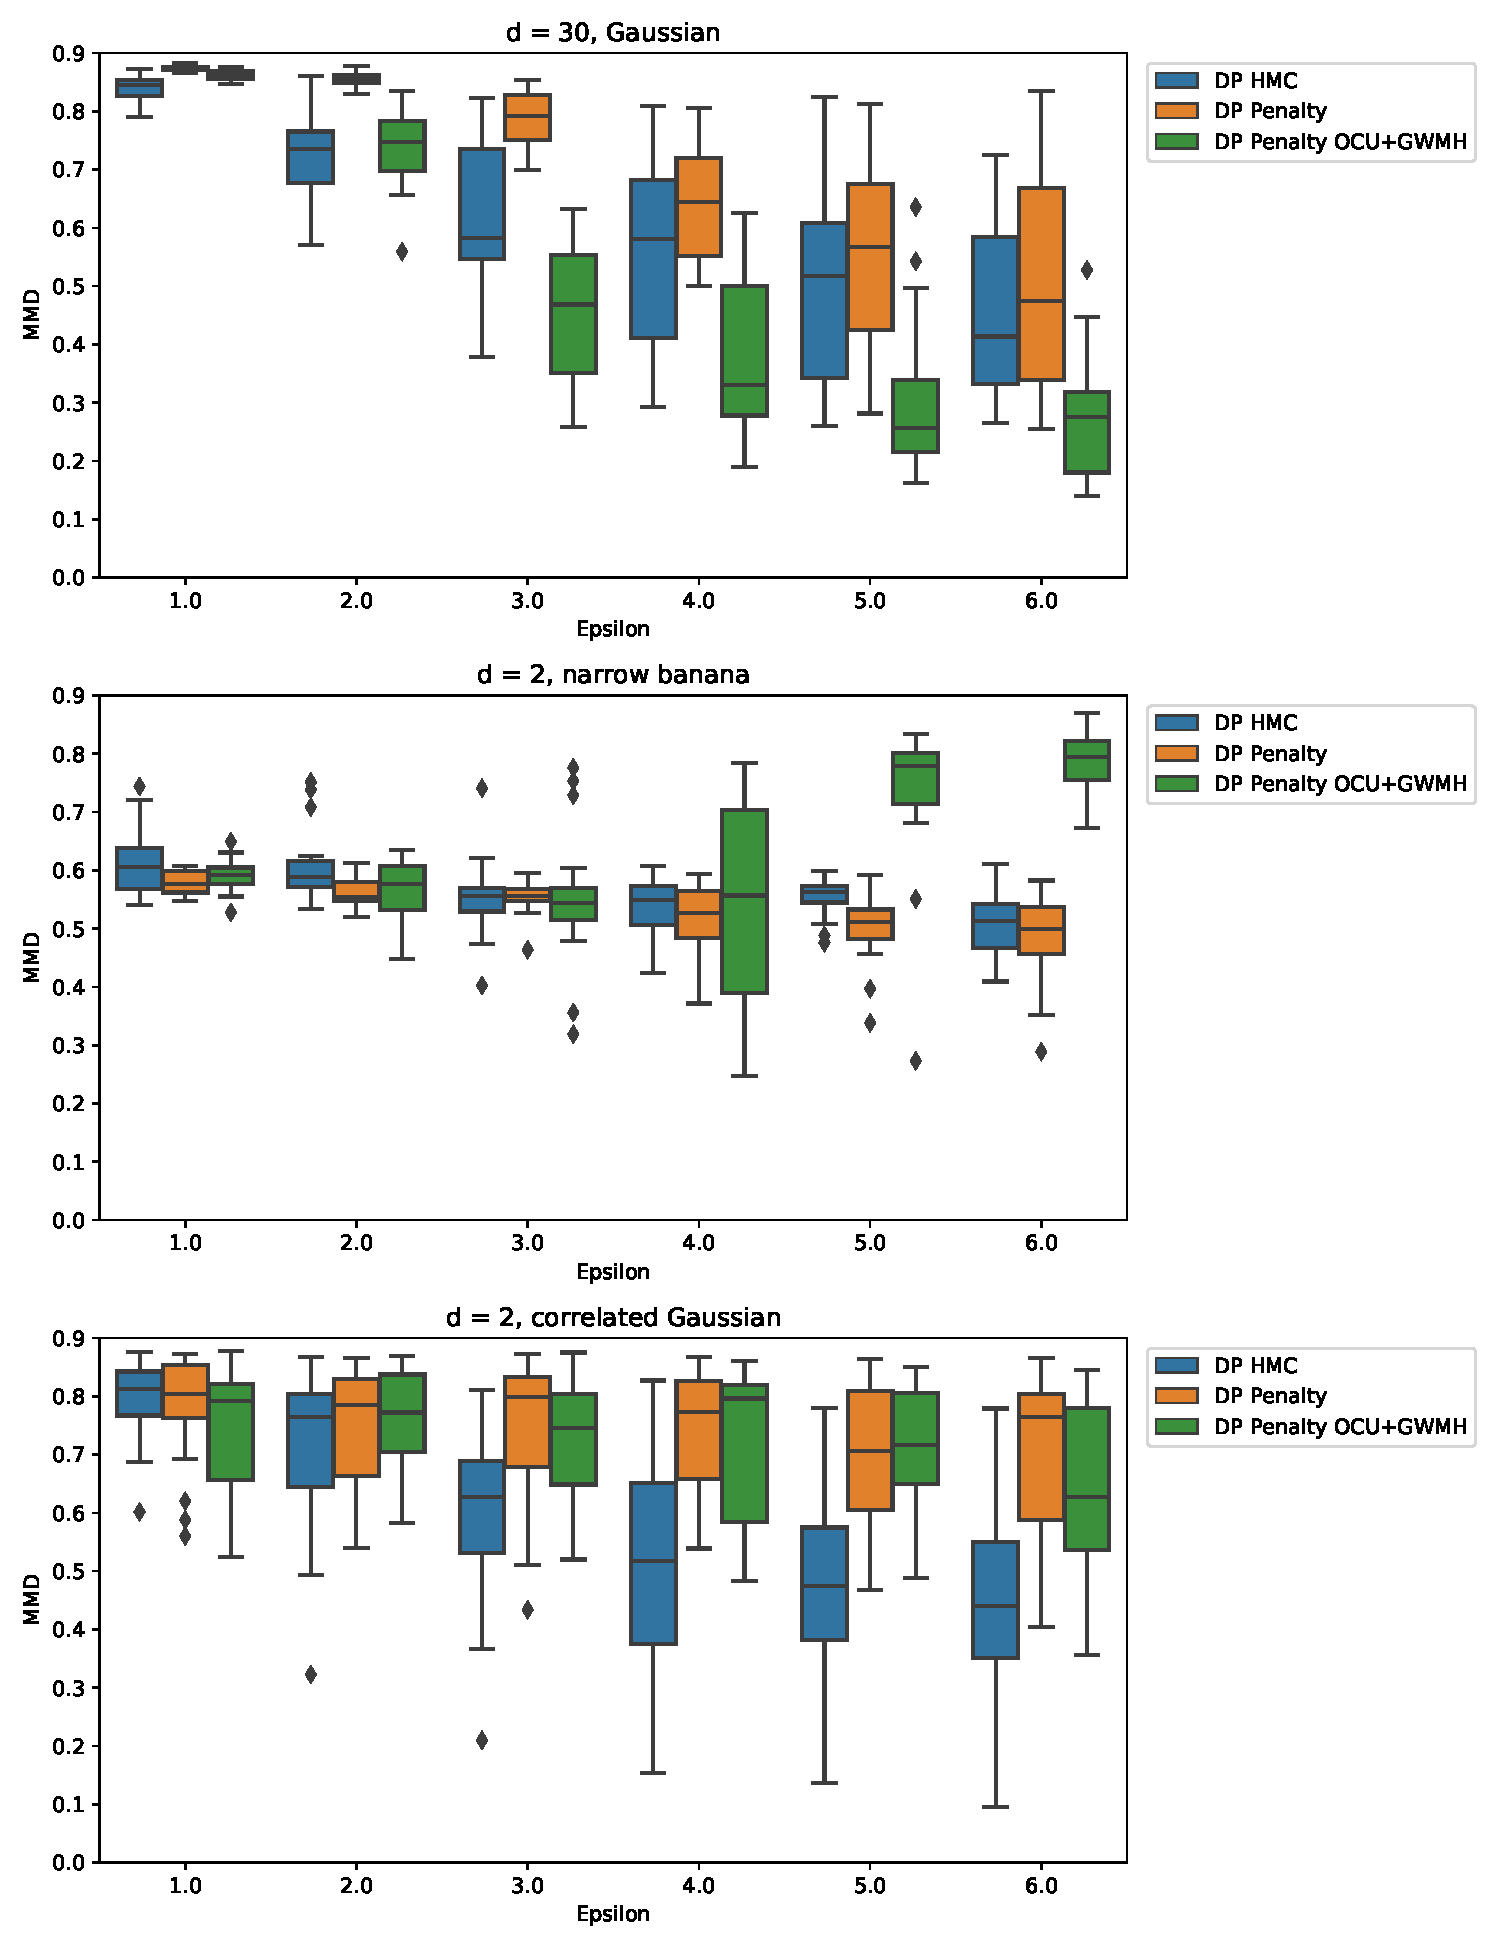
\includegraphics[width=\textwidth]{figures/banana_extra}
  \caption{Hard banana and Gaussian MMD}
  \label{banana_extra_mmd_fig}
\end{figure}
\begin{figure}[h]
  \centering
  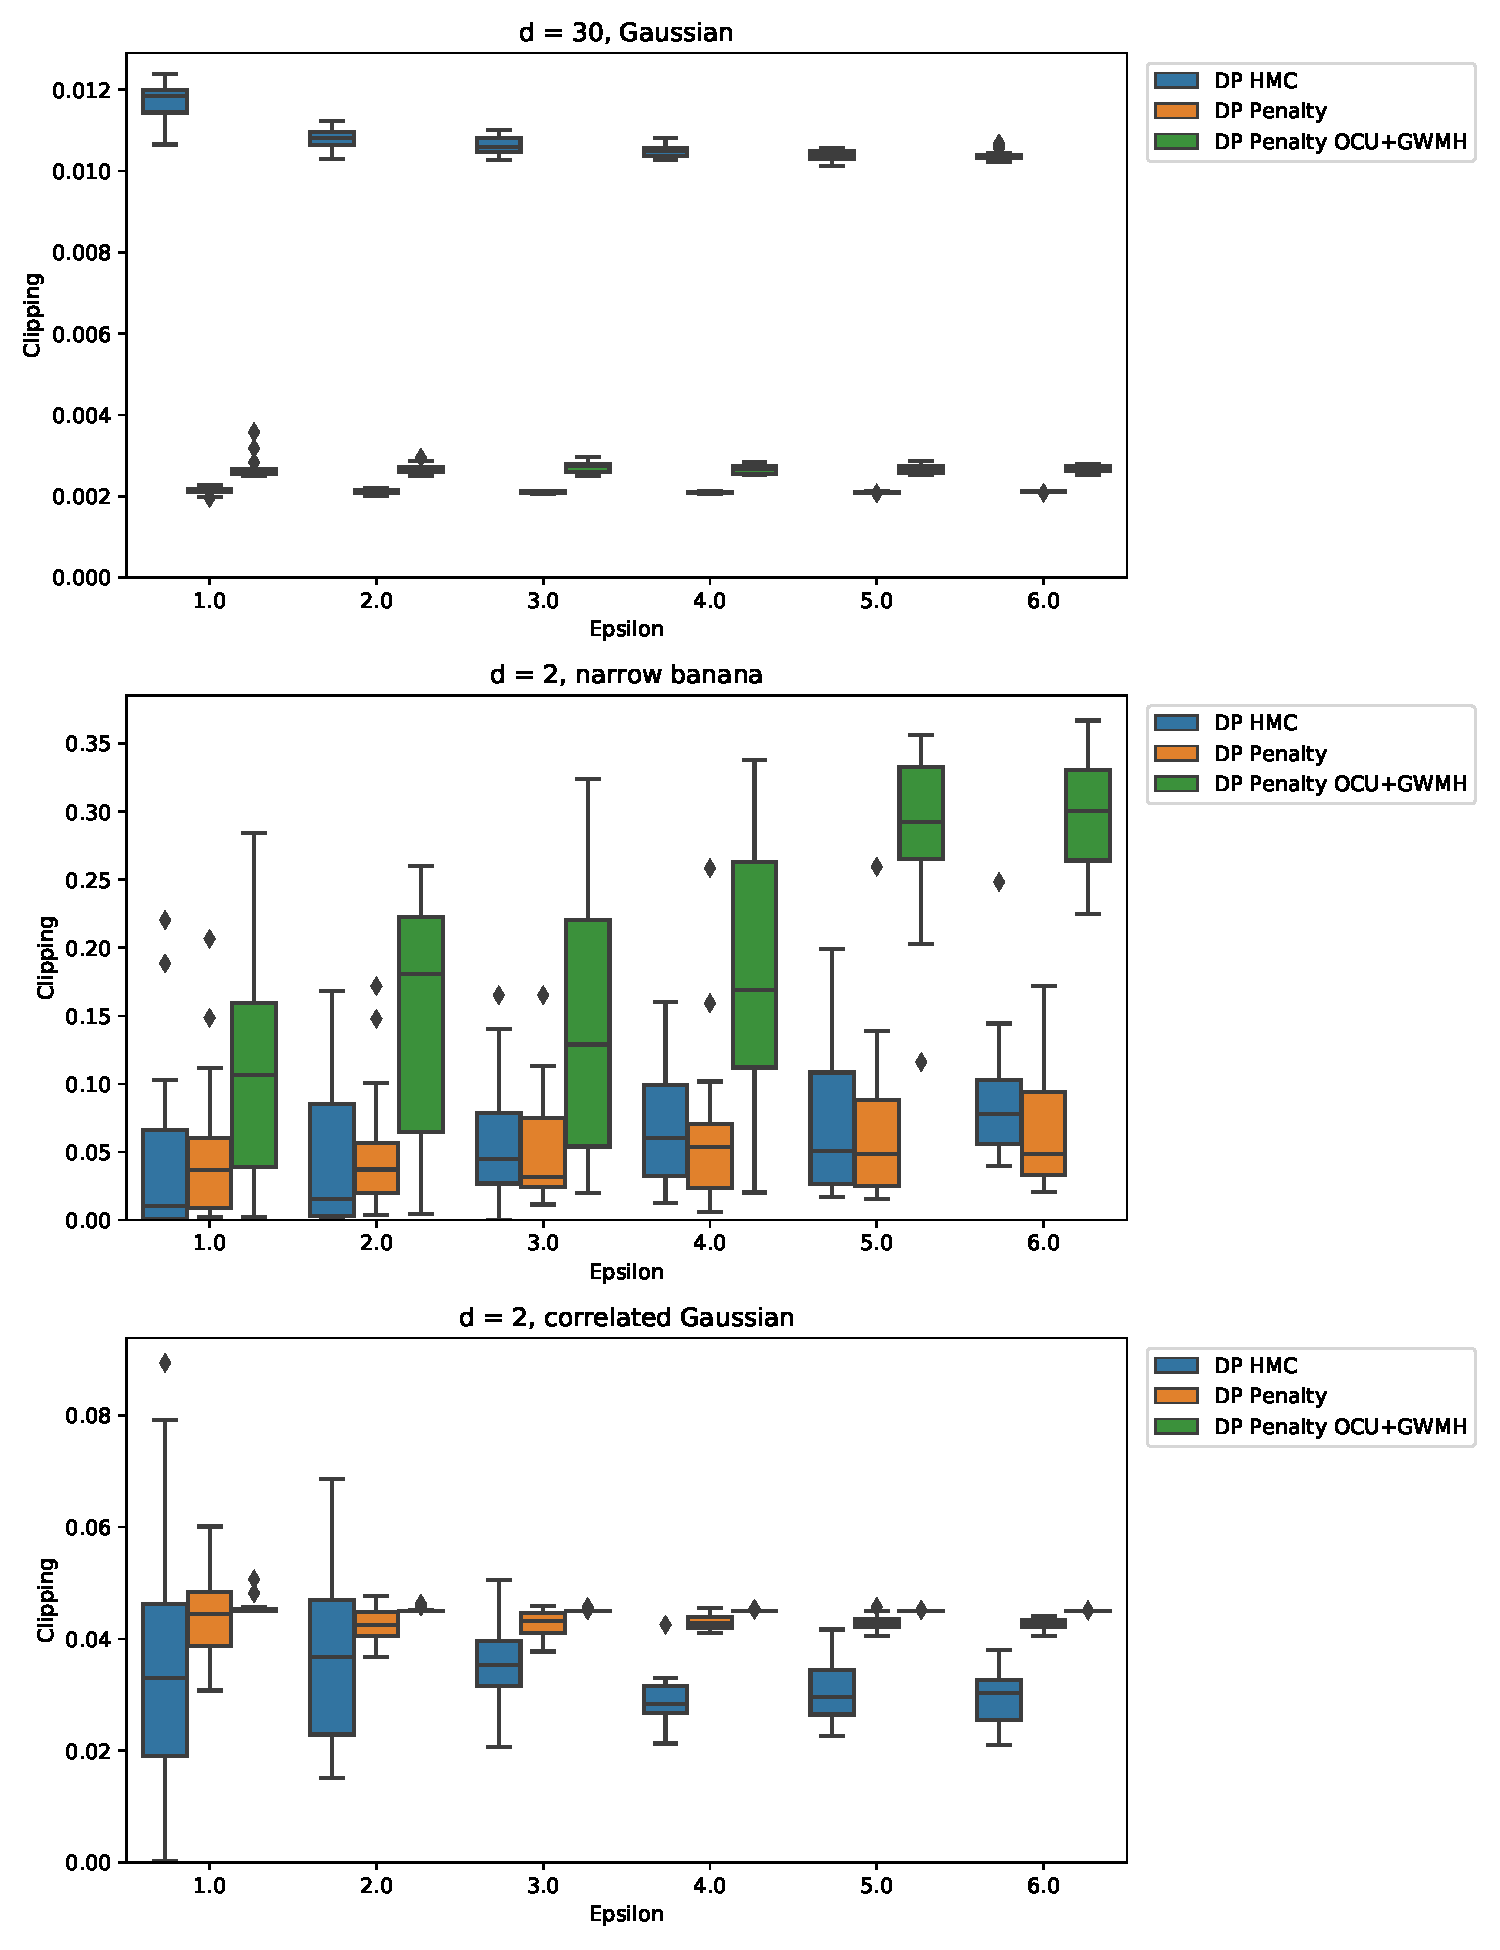
\includegraphics[width=\textwidth]{figures/banana_extra_clipping}
  \caption{Hard banana and Gaussian clipping}
  \label{banana_extra_clipping_fig}
\end{figure}
\begin{figure}[h]
  \centering
  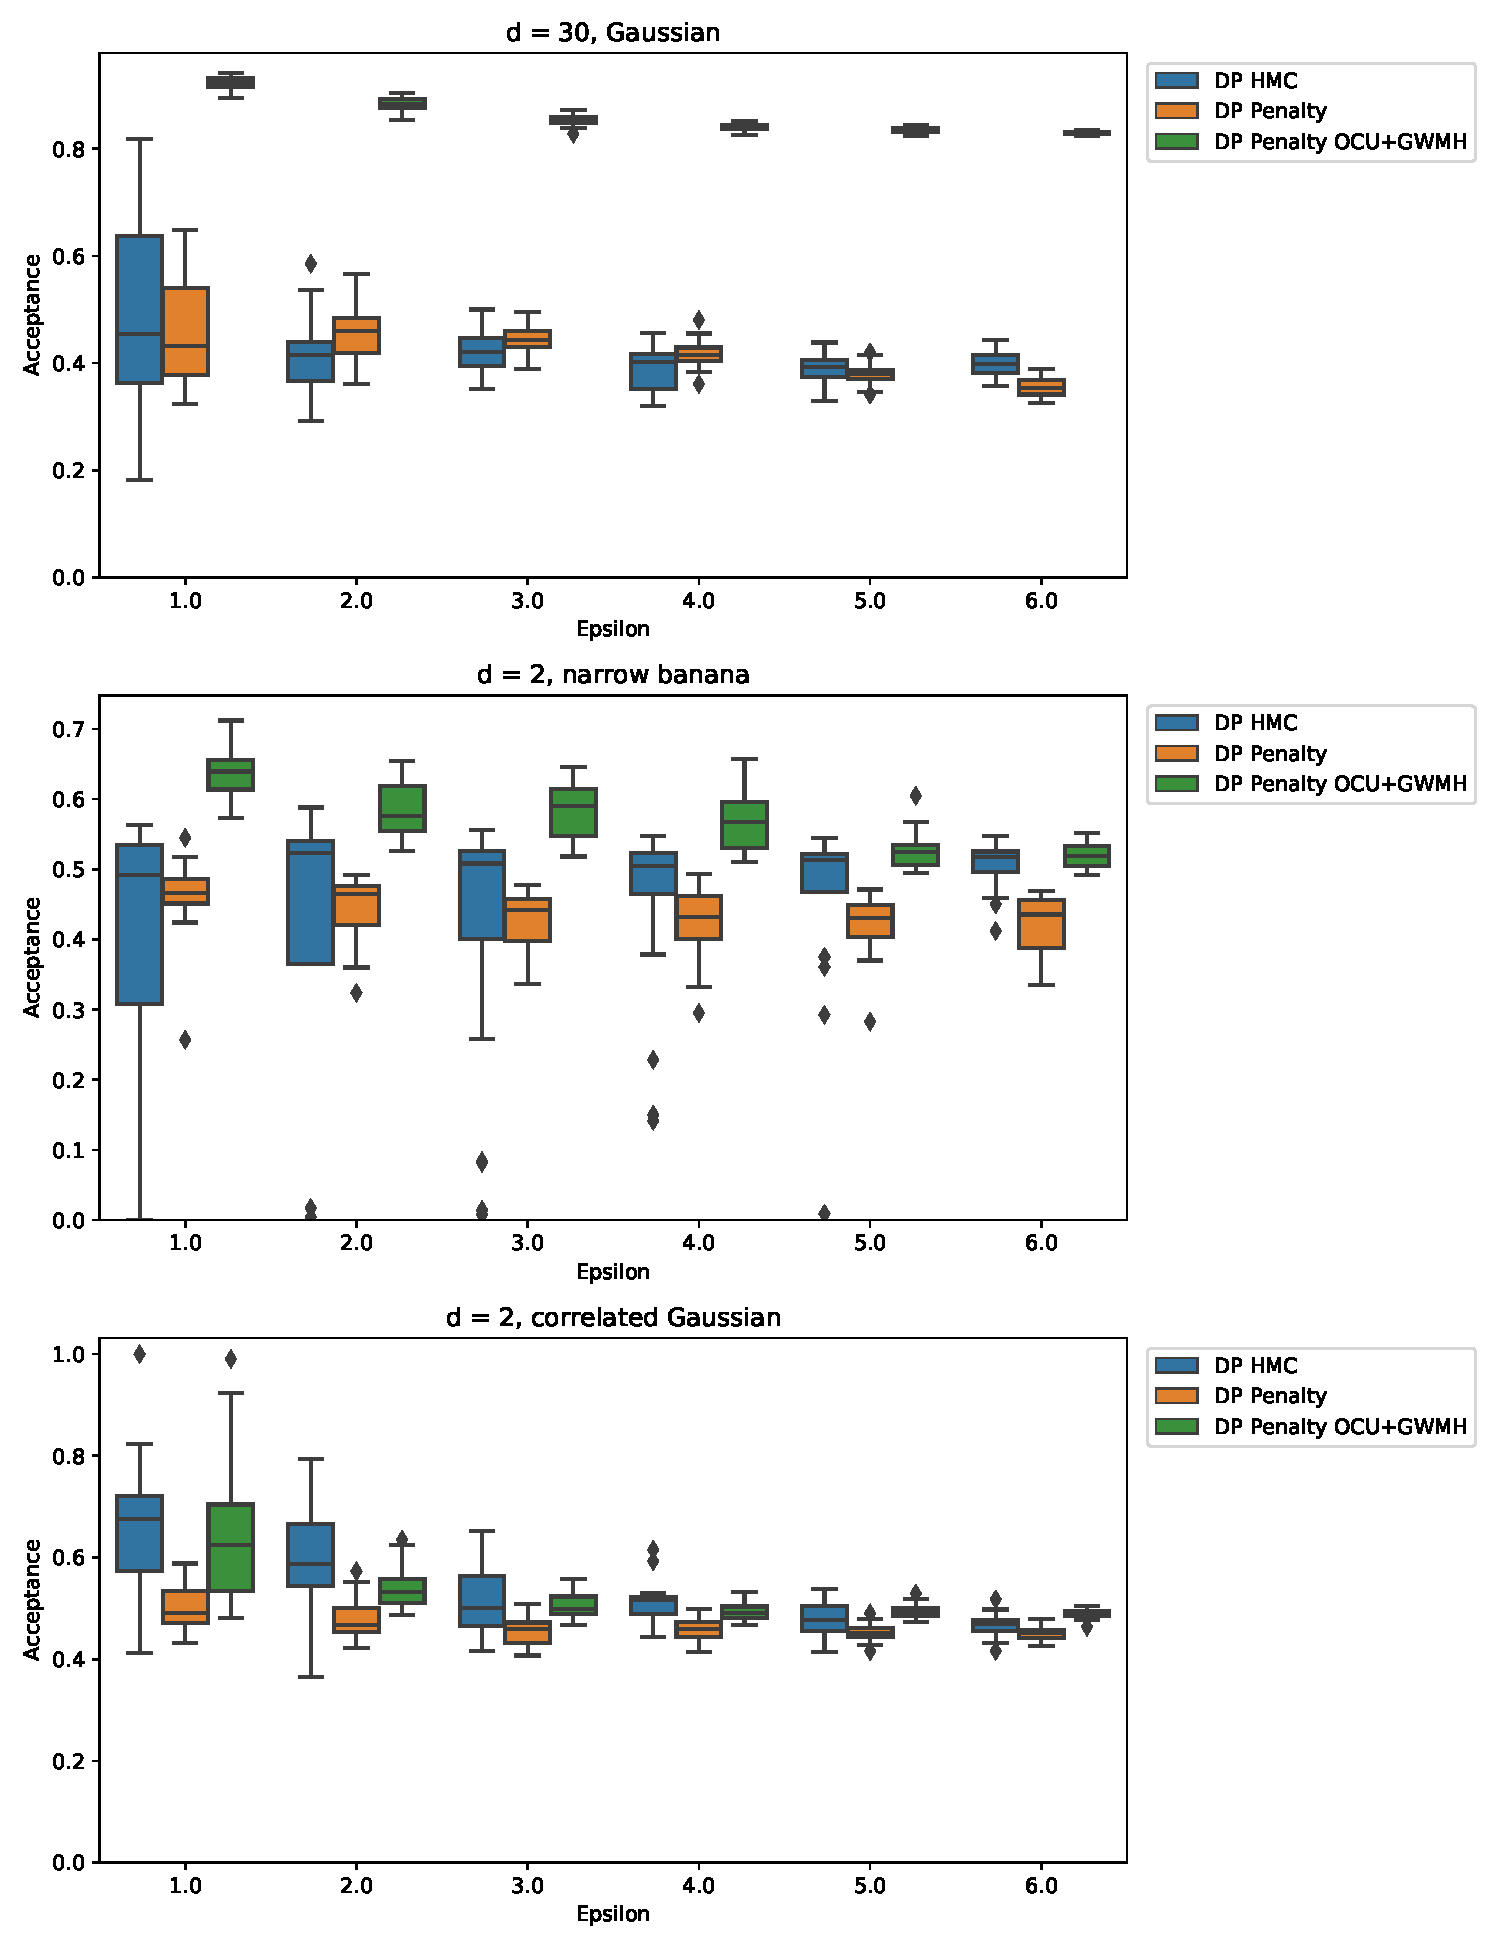
\includegraphics[width=\textwidth]{figures/banana_extra_acceptance}
  \caption{Hard banana and Gaussian acceptance rate }
  \label{banana_extra_acceptance_fig}
\end{figure}

Figure~\ref{banana_gradient_clipping_fig} shows the gradient clipping of
HMC for all the previous experiments. Gradient clipping does not affect
the convergence of HMC, so keeping it small it not as important as with
log likelihood clipping. However, gradient clipping does the acceptance rate
of HMC, but increasing the clip bound to lower clipping will increase the
noise added to gradients, thus also lowering the acceptance rate.

\begin{figure}[h]
  \centering
  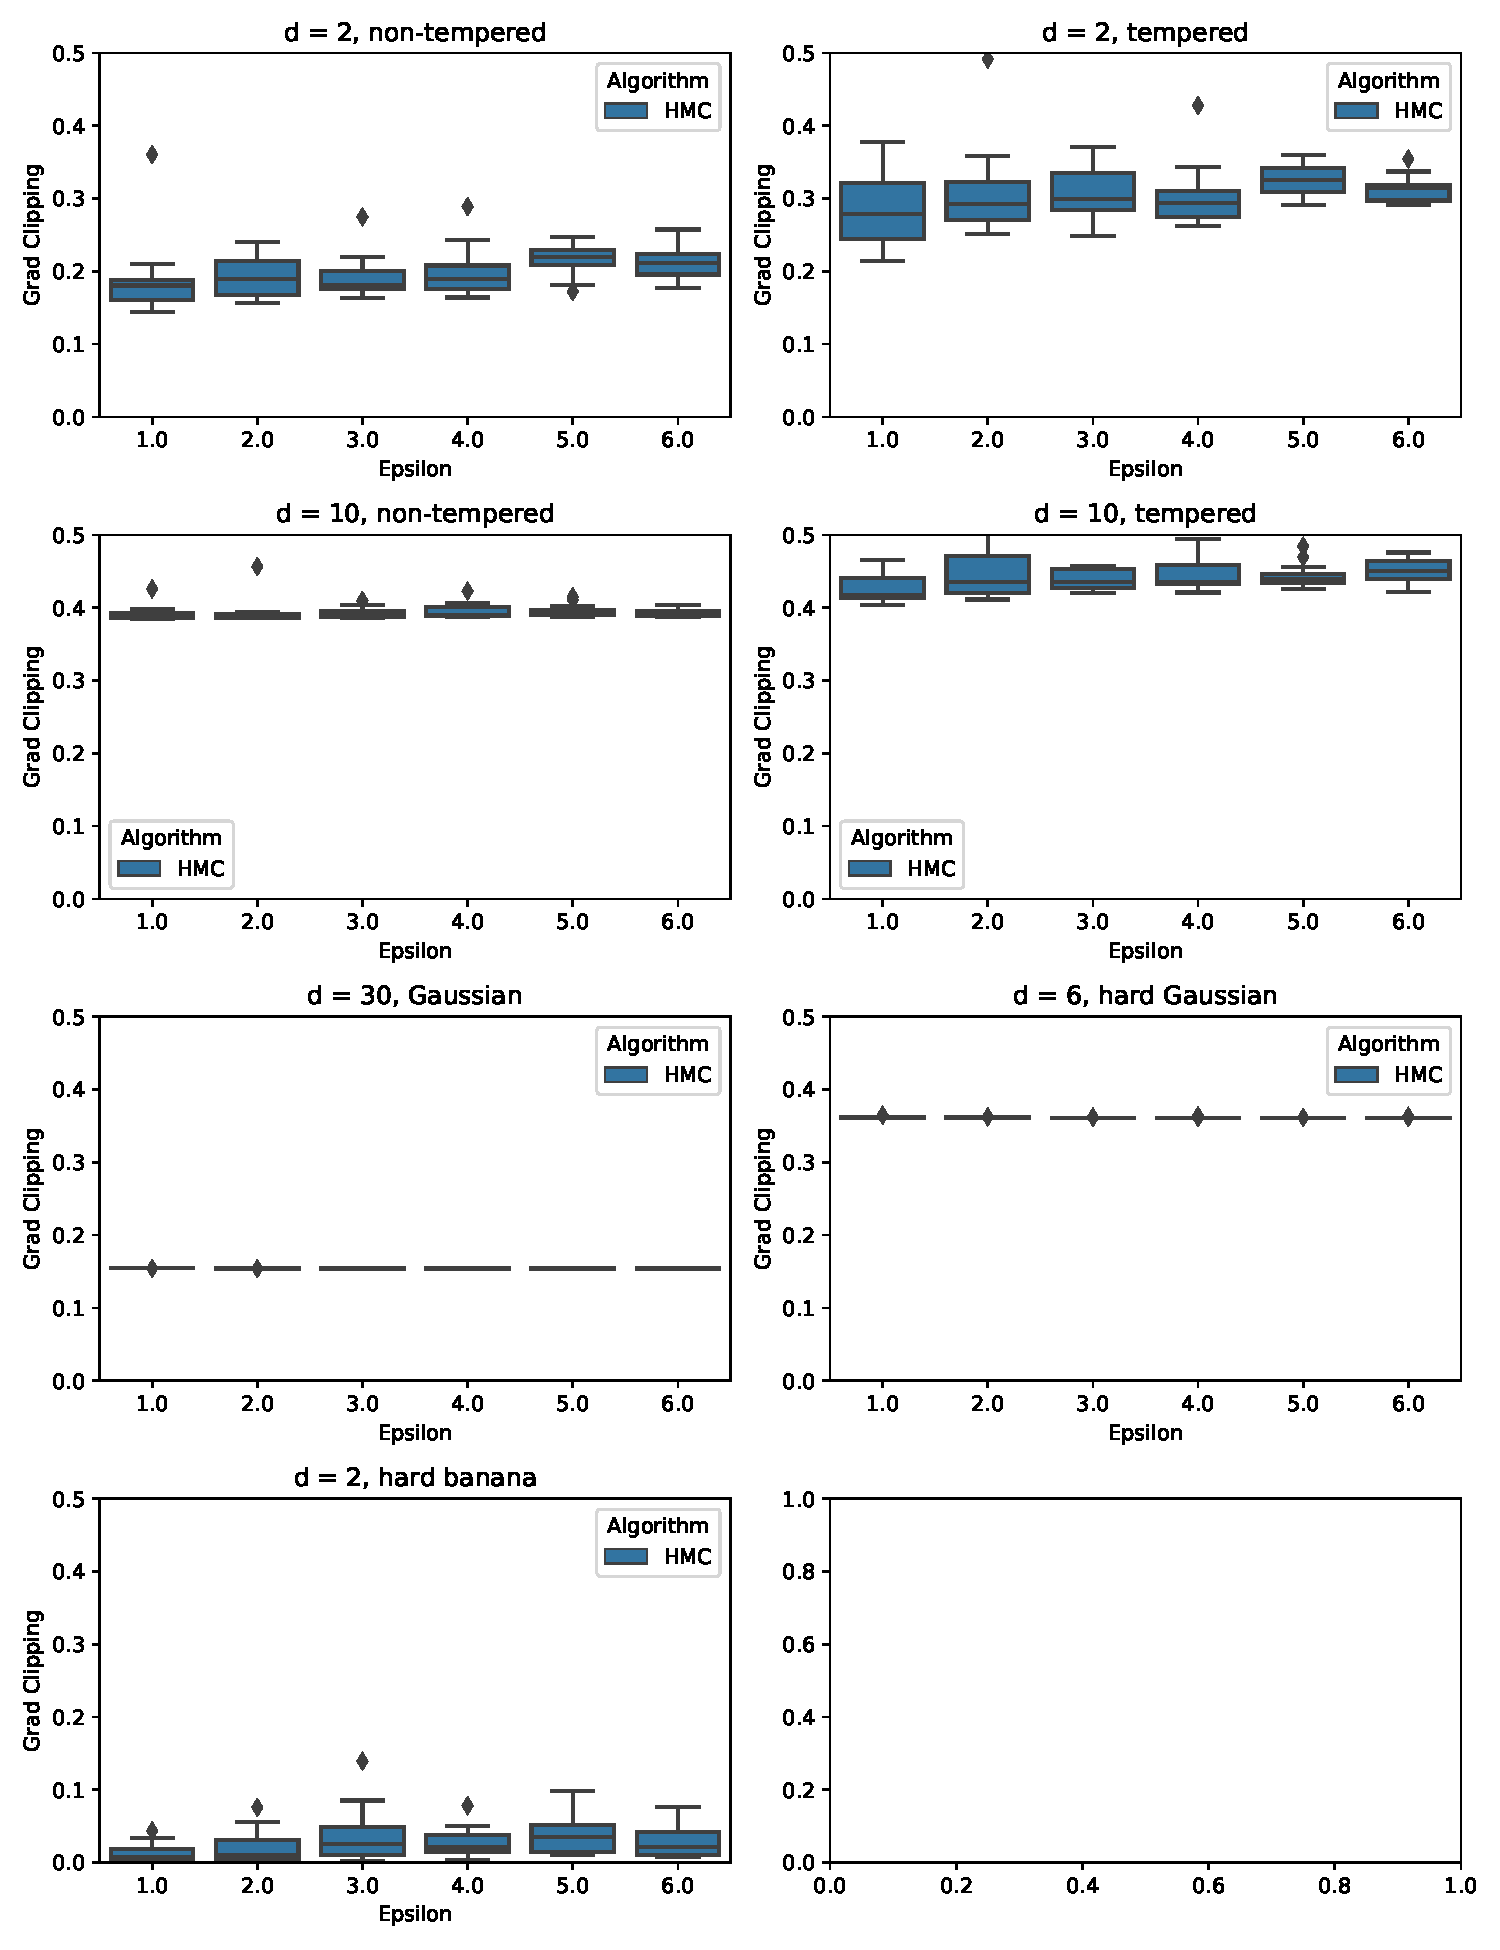
\includegraphics[width=\textwidth]{figures/banana_grad_clipping}
  \caption{Gradient clipping for HMC}
  \label{banana_gradient_clipping_fig}
\end{figure}

Finally, Figure~\ref{circle_fig} shows the distance from the posterior mean
to the true mean on the left, and clipping on the right, for the circle
experiment. Mean error was used instead of MMD, because in the circle model the
mean error measures how well the samples cover the entire ring of high probability
evenly, and the true mean can easily be shown to be 0.

With \(\epsilon = 0.5\) HMC outperforms DP penalty, but with larger
epsilons the differences disappear. This is likely due to both algorithms getting
close sampling from the true posterior with \(\epsilon = 1\).

\begin{figure}[h]
  \centering
  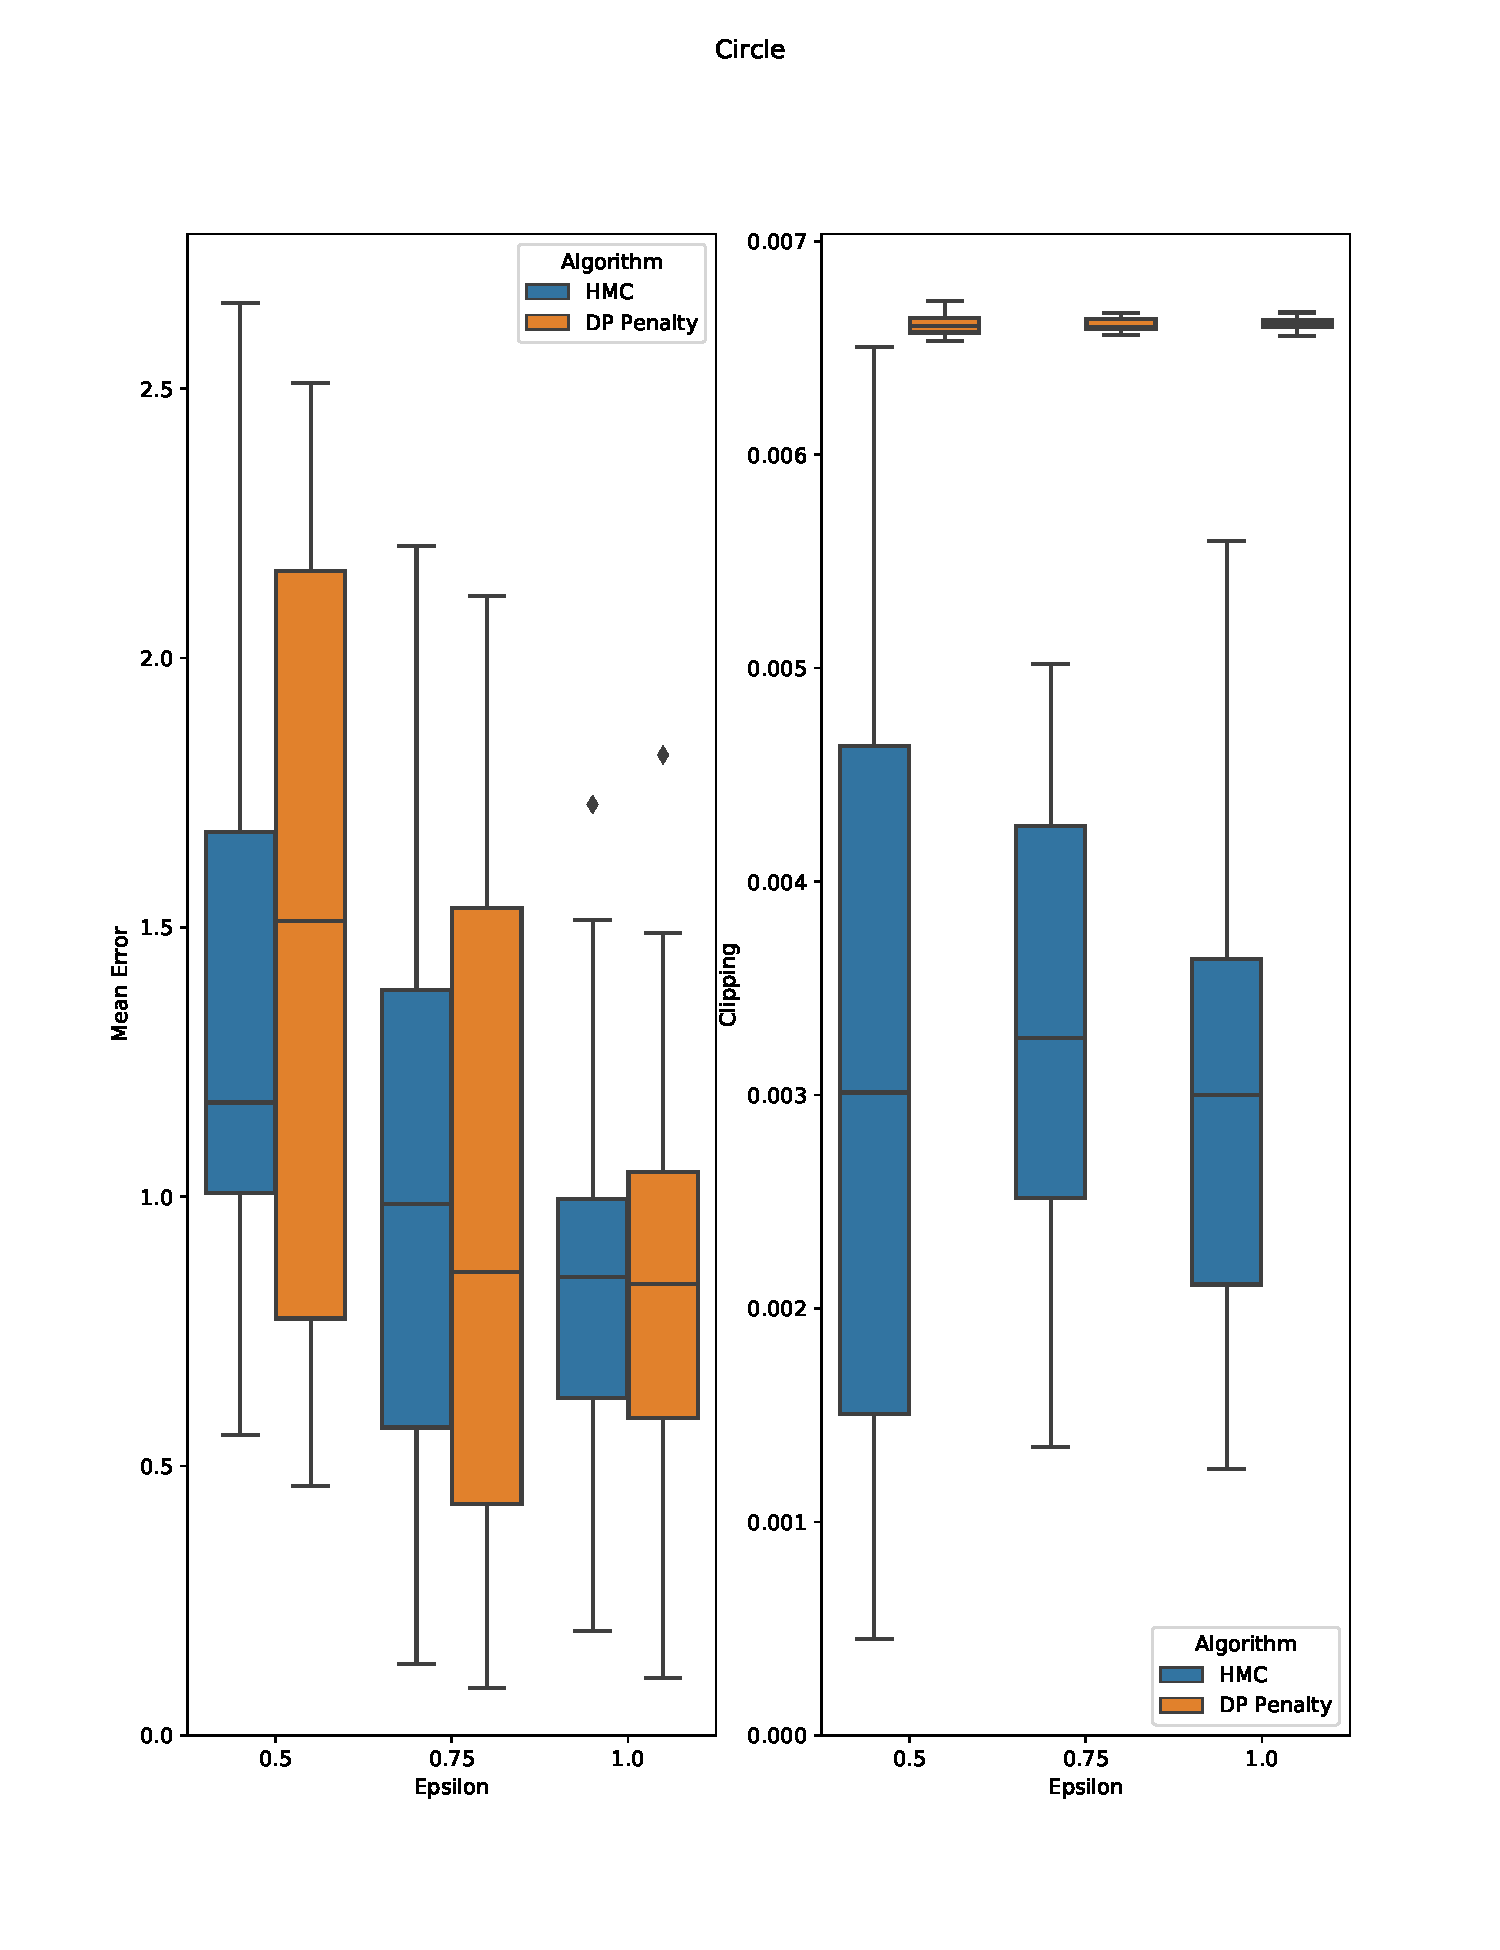
\includegraphics[width=\textwidth]{figures/circle.pdf}
  \caption{Circle experiment}
  \label{circle_fig}
\end{figure}

\printbibliography{}
\end{document}
